\chapter{Datasets}
\section{Dataset description}
\label{Dataset description}
Creating a high quality, well-balanced dataset is an essential step in the process of deepfake generation. Poorly prepared training set might cause that even great network architectures and state of the art algorithms will produce disappointing results. The most efficient approach to this problem ,in case of face-swapping technology, is obtaining images of targeted people from video recordings, which allows to produce great number of images that cover different facial expressions and head positions. There are several factors that should be taken into a consideration in order to construct proper dataset. First of all, videos of people with at least slight resemblance should be chosen. The most important feature in this matter is skin tone but the more similar appearances, the more deceiving deepfake might be achieved. Another important factor is overall quality of source material. Videos with high resolution and large number of frames per second are best suited for this purpose, but also require more computational power and time to properly train necessary networks. Finally, after a deconstruction of videos into single images, all set should be revised to remove pictures that depict faces which are blurry, deformed or in some ways covered, for example by hand.\\

For sake of this research the ``VoxCeleb2'' dataset was used. As described in \cite{voxceleb2_bib}, VoxCeleb2 consists of over 1 million utterances of over 6000 celebrities derived from videos from YouTube platform. Source data is diversified in terms of recorded people's genders, ethnicities, ages and accents, but also in terms of videos quality, lighting conditions, stability and lengths. Each recording has a resolution of 224 by 224 pixels and depicts closeup shot of a character's face and shoulders, which is close enough to clearly capture subtle facial expressions.

\begin{figure}[H]
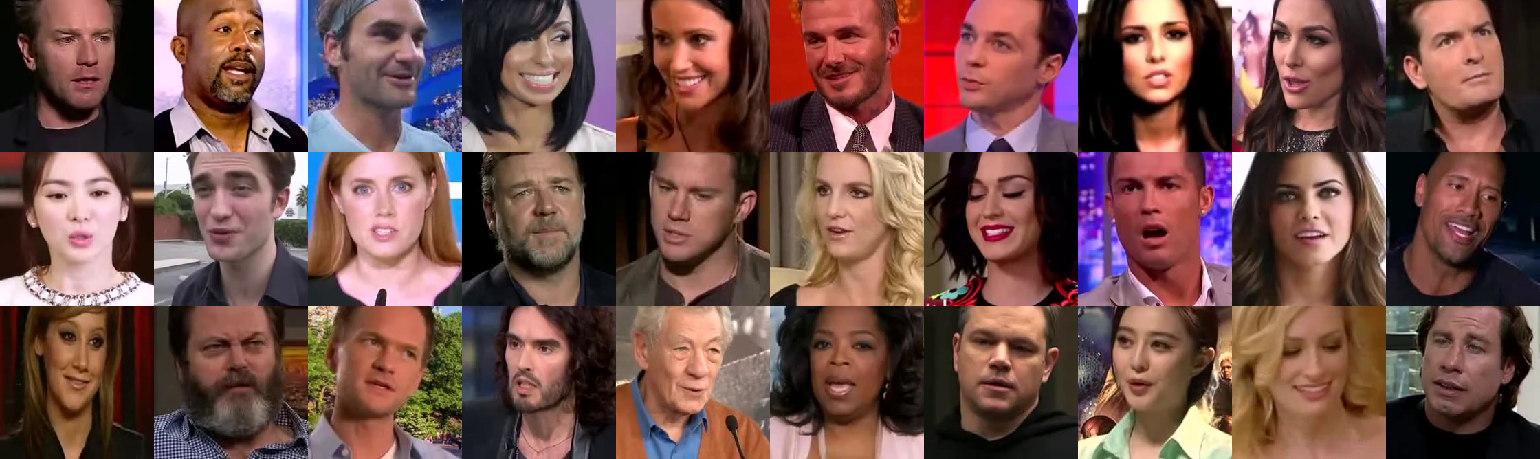
\includegraphics[width=14cm] {voxceleb2_sample.png}
\centering
\caption{Sample images from VoxCeleb2 dataset}
\label{fig:voxceleb2_sample}
\end{figure}

\section{Data pre-processing}
To prepare dataset best suited for purpose of this research following preparations were made, in accordance with guidelines described in section \ref{Dataset description}. Sample images of pre-processed data are presented in figure \ref{fig:subjects_sample}.

\begin{enumerate}
\item Two actors (Leonardo DiCaprio and Robert Downey Jr.), further called subject A and subject B, were chosen as targets of face replacement. This choice was dictated by how well their faces are known and recognizable which facilitates the final assessment and by factors mentioned in section \ref{Dataset description}.

\item From the set of all videos of chosen subjects, available in ``VoxCeleb2'' dataset, those which presented subjects in similar age and had good recording quality were selected.

\item From each video every tenth frame was extracted to limit the amount of nearly identical images. Additionally, through Haar feature-based cascade classifiers described in section \ref{Haar feature-based cascade classifiers}, the face itself was cut out from each extracted frame to discard unnecessary parts of pictures.

\item Resolutions of all obtained face images varied, therefore data had to be rescaled to a common resolution of 160 by 160 pixels.

\item Final step, was to save obtained images as arrays into a single file in uncompressed ``.npz'' format. This allows easy data transferring and simplifies the process of loading data during the training of artificial neural networks.
\end{enumerate}

\begin{figure}[H]
\centering
\begin{subfigure}{.5\textwidth}
  \centering
  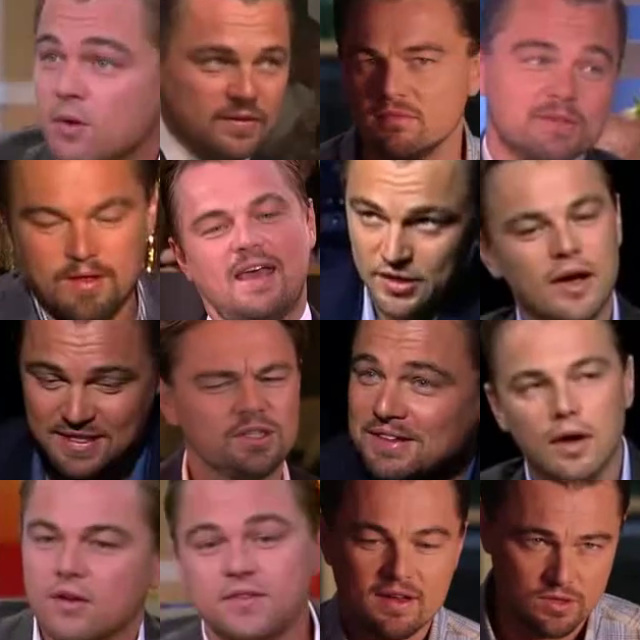
\includegraphics[width=0.9\linewidth]{dicaprio_sample.png}
  \caption{Sample images of subject A}
  \label{subfig:subject_A_sample}
\end{subfigure}%
\begin{subfigure}{.5\textwidth}
  \centering
  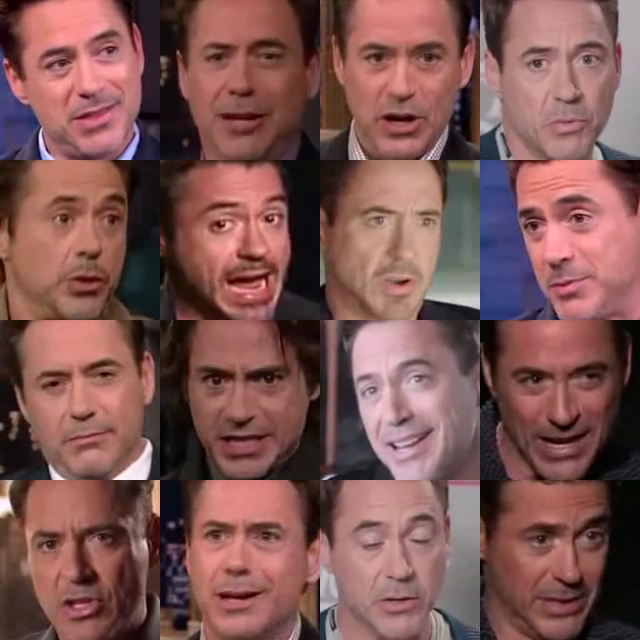
\includegraphics[width=0.9\linewidth]{downeyjr_sample.png}
  \caption{Sample images of subject B}
  \label{subfig:subject_B_sample}
\end{subfigure}
\caption{Sample images of pre-processed data}
\label{fig:subjects_sample}
\end{figure}
